\section{The Models}
\label{sec:models}

Real-time tracking applications such as ours often use
a Bayesian filtering approach,
or recursive Bayesian estimation,
in which the data is processed sequentially instead of all at once,
reducing computational demands.
These models assume an underlying Markov process with state $\mathcal{X}_k$
and system noise $\omega_k\sim\mathrm{N}(0,\mathcal{Q})$ 
of which observations $\mathcal{Y}_k$ are made
with error $\nu_k\sim\mathrm{N}(0,\mathcal{R})$,
giving the following general model:
\begin{equation}
\label{eq:rbe_model}
\begin{split}
\mathcal{X}_k &= f(\mathcal{X}_{k-1}, \omega_k) \\
\mathcal{Y}_k &= h(\mathcal{X}_k, \nu_k)
\end{split}
\end{equation}
The transition function $f$ describes the relationship between consecutive states,
while the measurement function $h$ is a deterministic function describing the
relationship between the underlying and observed states.

The following sections describe the two models used in this application,
both of which are examples of a Bayesian filter.
The first, implemented using a particle filter, estimates vehicle states
to infer travel times along roads from a sequence of GPS positions;
the second uses these travel times to update road states 
and is implemented using an \emph{information filter},
a variant of the Kalman filter \citep{Anderson_2012}.

\subsection{Real-time vehicle model}
\label{sec:pf}

The underlying vehicle state at time $t_k$ consists of
the vehicle's distance traveled $x$ in meters along the route and
its speed $\dot x$ in meters per second.
Additionally, travel times along road segments along the route, 
$\bz = (z_1,\ldots,z_L)^\top$, in seconds,
are included in the state and estimated
sequentially as the vehicle traverses the route.
These are combined into the state vector,
\begin{equation}
\label{eq:vehicle_state}
\bX_k = 
\begin{bmatrix}
    x_k \\ \dot x_k \\ \bz
\end{bmatrix}.
\end{equation}
Observations $\bY_k$ of the vehicle are made using a GPS at time $t_k$
with GPS error $\epsilon^2$,
giving the longitude $\lambda_k$ and latitude $\phi_k$ of the vehicle,
\begin{equation}
\label{eq:vehicle_obs}
\bY_k = \begin{bmatrix} \lambda_k \\ \phi_k \end{bmatrix}.
\end{equation}


We chose to employ a particle filter to estimate $\bX_k$,
due to do its high flexibility and use in recent 
transit vehicle modeling applications \citep{Hans_2015}.
The primary advantage of a particle filter is its handling of multimodality,
as demonstrated in figure~\ref{fig:pf_state_predict},
which is a common feature of the proposal distribution, particularly around bus stops.
Another advantage is the intuitive likelihood function (see section~\ref{sec:pf_update}).
Conversely, particle filter methods are computationally demanding,
requiring an increasing number of particles as the model complexity and
number of parameters increases \citep{Carpenter_1999}.
Section~\ref{sec:rt} describes our implementation of the particle filter in real-time 
and its timings.



\begin{figure}[tb]
    \centering
    \begin{subfigure}[t]{0.48\textwidth}
        \centering
        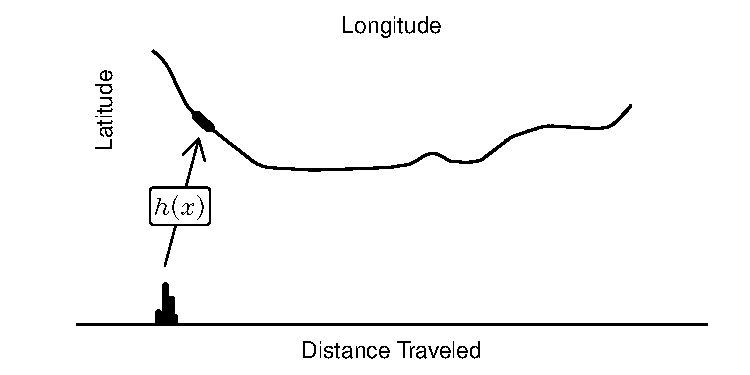
\includegraphics[width=\textwidth]{figures/03_particle_filter_1.pdf}
        \caption{The vehicle state represented by a sample of discrete points is related to the observable state (GPS position) through the transition function $h$.}
        \label{fig:pf_state_prev}
    \end{subfigure}\;\;
    \begin{subfigure}[t]{0.48\textwidth}
        \centering
        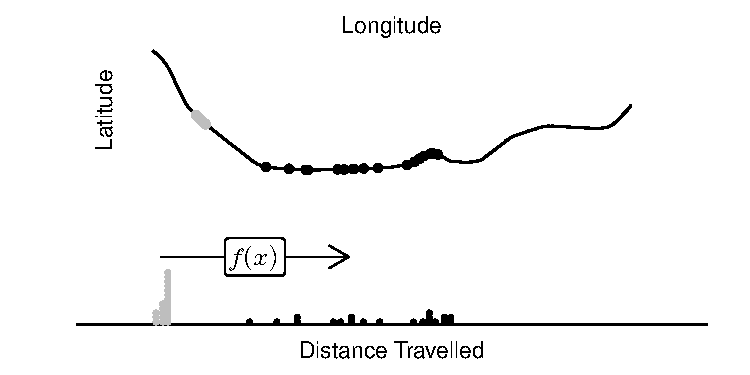
\includegraphics[width=\textwidth]{figures/03_particle_filter_2.pdf}
        \caption{The transition function $f$ models the behaviour of each particle,
            including changes in acceleration and stopping behaviour at bus stops,
            which can result in multiple modes.}
        \label{fig:pf_state_predict}
    \end{subfigure}\\
    \begin{subfigure}[t]{0.48\textwidth}
        \centering
        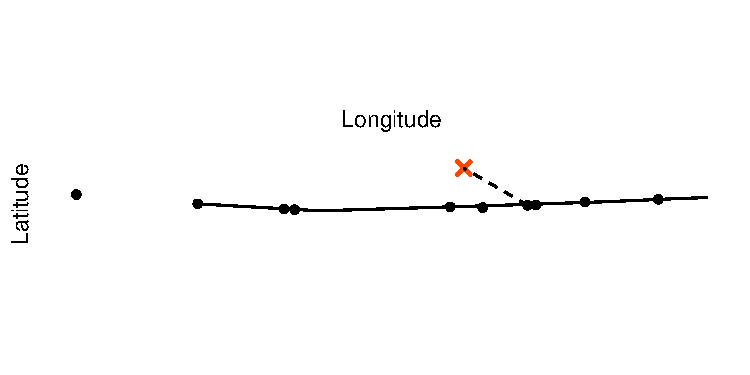
\includegraphics[width=\textwidth]{figures/03_particle_filter_6.pdf}
        \caption{Each particle's distance from the true observation (red cross) 
            is calculated using
            the geographic distance between two coordinates, which can then be used
            to calculate it's weight.}
        \label{fig:pf_state_update}
    \end{subfigure}\;\;
    \begin{subfigure}[t]{0.48\textwidth}
        \centering
        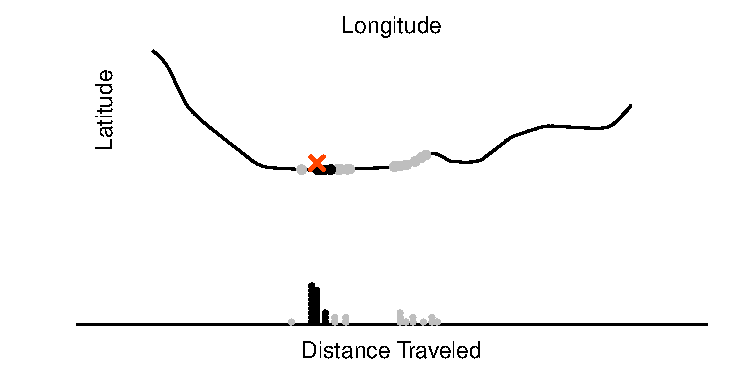
\includegraphics[width=\textwidth]{figures/03_particle_filter_4.pdf}
        \caption{Resampling occurs using likelihood weights that use the distance
            between the particle's location and the vehicles reported location (red cross),
            resulting in the updated state.}
        \label{fig:pf_state_predict2}
    \end{subfigure}
    \caption{The vehicles state is estimated using a set of discrete points, or particles,
        each of which is independently mutated to make predictions of the future state.
        Multimodality is easily handled, as demonstrated here,
        without degeneration of the filter.}
    \label{fig:pf_state}
\end{figure}




In a particle filter, the posterior distribution of the state at time $t_{k-1}$
is represented by a set of discrete points, or particles, (Figure~\ref{fig:pf_state_prev}),
each with an associated weight $W_{k-1}^{(i)}$
\begin{equation}
p(\bX_{k-1} | \bY_{k-1}) \approx \tilde\bX_{k-1|k-1} 
:= \left\{\bX_{k-1}^{(i)}, W_{k-1}^{(i)}\right\}_{i=1}^N
\end{equation}
each of which is independently updated or \emph{mutated} using the transition function $f$ (fig~\ref{fig:pf_state_predict})
\begin{equation}
p(\bX_k | \bX_{k-1}) \approx \tilde\bX_{k|k-1} := 
\left\{f(\bX_{k-1}^{(i)}, \psi), W_{k-1}^{(i)}\right\}_{i=1}^N
\end{equation}
using parameter vector $\psi$ containing all of the necessary parameters
for the model (including system noise).
After mutation, 
the state is updated by reweighting the particles using the likelihood $p(\bY_k | \bX_k^{(i)})$ 
(sec.~\ref{sec:pf_update}) and standardising so $\sum_{i=1}^N W_k^{(i)} = 1$,
\begin{equation*}
W_k^{(i)} = \frac{W_{k-1}^{(i)} p(\bY_k | \bX_k^{(i)})}{
    \sum_{j=1}^N W_{k-1}^{(j)} p(\bY_k | \bX_k^{(j)})
}
\end{equation*}
generating a posterior estimate of the state
\begin{equation}
p(\bX_k | \bY_k) \approx \tilde\bX_{k|k} := 
\left\{\bX_{k}^{(i)}, W_{k}^{(i)}\right\}_{i=1}^N.
\end{equation}

In order to prevent degeneration of the particle filter state,
\emph{importance resampling} is employed whenever the 
effective sample size 
\begin{equation}
\label{eq:neff}
N_{\text{eff}} = \frac{1}{\sum_i (W_k^{(i)})^2}
\end{equation}
falls below a specified threshold $N_{\text{thres}}$.
The resampling is performed with replacement using importance weights $W_k^{(i)}$,
as demonstrated in Figure~\ref{fig:pf_state_predict2}.
Afterwards, the weights are reinitialized to $W_k^{(i)} = N^{-1}$.
Note this is a computationally demanding step,
so reducing the rate of resampling is favourable.



\subsubsection{Vehicle transition function}
\label{sec:pf_prediction}

The particle filter allows us to develop a model of several important bus behaviours:
\begin{itemize}
\item non-constant speed along roads,
\item optional stopping and waiting at bus stops while passengers board and disembark, and
\item optional stopping and waiting at intersections or traffic lights (future work).
\end{itemize}

For each particle, the transition function generates a plausible trajectory,
using system noise parameter $\sigma^2$ which describes 
how the vehicle's acceleration changes as a Markov process.
The vehicle does not travel constantly along the route,
however, as it needs to service bus stops along the way,
so the transition function includes 
stopping probabilities $\boldsymbol\pi = (\pi_1,\ldots,\pi_J)^\top$ at bus stops,
dwell times $\boldsymbol\tau = (\tau_1,\ldots,\tau_J)^\top$ for passengers to
board and disembark (conditional on the bus stopping),
and the minimum dwell time at stops, $\gamma$,
for the doors to open and close,
and account for deceleration and acceleration.
For these parameters, we used constant values for all stops,
based on the values used by \cite{Hans_2015};
future work will investigate modeling these in real-time similarly to Section~\ref{sec:kf}.

The stop positions are represented by their distance into trip,
$\boldsymbol{S} = (S_1, \ldots, S_J)^\top$.
The $stop\_index$ function returns the index of a stop,
given a distance traveled and set of stop distances.
The transition function algorithm is shown in Algorithm~\ref{fig:algorithm},
which implements those features discussed above.
Lines~2--9 are necessary to decrease the degeneration rate of the filter,
which can occur when there is a long delay between observations
simply because the bus has not moved due to traffic or other reasons. 
We therefore place positive probability for some particles to remain stationary.

Lines~11--12 of Algorithm~\ref{fig:algorithm} implement the system noise,
which involves changing the vehicle's speed each second (i.e., acceleration).
Lines~13--25 handle arrival behaviour at stops:
if the particle passes the next stop,
it has a chance of stopping (lines~18--19),
in which case the dwell time is sampled and deducted from the 
time remaining to travel (lines~20--21).
Finally, to track travel time along segments,
at each point where the vehicle travels (lines 9 and 26),
the travel time for that segment, $z_j$, is incremented.
The mutation ends once the travel time $\delta$ reaches zero,
or when the vehicle reaches the end of the route (lines 10, 14).
Once finished, the particle's new state is returned (line 29).

\renewcommand{\algorithmicrequire}{\textbf{Start:}}
\newcommand{\algorithmicbreak}{\textbf{break}}
\newcommand{\Break}{\State \algorithmicbreak}
\begin{algorithm}[tb]
    \caption{Particle mutation function.}
    \label{fig:algorithm}
    \begin{algorithmic}[2]
    \Require $x_{k-1}, \dot x_{k-1}, \boldsymbol z$\\
    Initialization $\delta \gets t_k - t_{k-1}$, 
        $j \gets stop\_index(x, \boldsymbol{S})$
    \If {$u \sim \mathrm{U}(0,1) < 0.5$ and $x = S_j$}
        \Comment{Remain longer at stop}
        \State $d_j \sim \mathrm{Exp}(1/\tau_j)$
        \State $\delta \gets \delta - \gamma - d_j$
    \ElsIf {$u \sim \mathrm{U}(0,1) < 0.1$}
        \Comment{Occasionally bus stopped due to traffic}
        \State $w \gets \min(\delta, \mathrm{Exp}(1/\delta))$
        \State $\delta \gets \delta - w$
        \State $z_j \gets z_j + w$
        \Comment{Congestion counts as travel time}
    \EndIf
    \While {$\delta > 0$ and $x < S_J$} 
        \State $\dot x \sim \mathrm{N}(\dot x, \sigma^2)$
        \Comment{System noise, trunctated to be non-negative}
        \State $x \leftarrow x + \dot x$
        \If {$x \geq S_{j+1}$}
            \If {$j+1 = J$}
                \Comment{Break at end of route}
                \State $x \gets S_J$
                \Break
            \EndIf
            \State $u_j \sim \mathrm{U}(0,1)$
            \Comment{Simulate vehicle stopping}
            \If {$u_j < \pi$}
                \State $d_j \sim \mathrm{Exp}(1/\tau_j)$
                \State $\delta \gets \delta - \gamma - d_j$
                \State $x \gets S_j$
            \EndIf
            \State $j\gets j+1$
        \EndIf
        \State $\delta \gets \delta - 1$
        \State $z_j \gets z_j + 1$
        \Comment{Track travel time along road}
    \EndWhile
    \\
    \Return $x, \dot x, \boldsymbol z$
    \end{algorithmic}
\end{algorithm}



\subsubsection{Updating state using the observation likelihood}
\label{sec:pf_update}

After mutating the particle set, the posterior distribution $\tilde\bX_{k|k}$ 
is obtained by reweighting each particle using the likelihood.
The measurement function $h$,
and an additional function $g$ which transforms GPS coordinates onto a flat
surface (the geographical equirectangular projection, \cite{Snyder_1998}),
allow the placement of a bivate normal likelihood on the data.
The model for the observations is,
assuming GPS error $\epsilon^2$,
\begin{equation}
\label{eq:pf_obs_model}
g(\bY_k) = g(h(\bX_k)) + \br_k,
\quad \br_k \sim \mathrm{N}(\boldsymbol{0}, \epsilon^2\boldsymbol{I})
\end{equation}
Now, the geographical distance between the observation and the true vehicle can be expressed
in terms of two independent random variables $z_1, z_2 \sim \mathrm{N}(0,1)$
\begin{equation}
\label{eq:obs_dist}
dist(\bY_k, h(\bX_k)) = \sqrt{r_{k1}^2 + r_{k2}^2} 
    = \sqrt{(\epsilon z_1)^2 + (\epsilon z_2)^2}.
\end{equation}
The sum of two independent, standard normal random variables 
is $\chi^2$ distributed with 2~degrees of freedom,
which is itself exponential,
so rearranging (\ref{eq:obs_dist}) yields
\begin{equation}
\label{eq:obs_exp}
\left(\frac{dist(\bY_k, h(\bX_k))}{\epsilon}\right)^2 =
z_1^2 + z_2^2 \sim \mathrm{Exp}\left(\frac{1}{2}\right)
\end{equation}

The likelihood of the data given a particle's state estimate 
cane be calculated using (\ref{eq:obs_exp})
\begin{equation}
p(\bY_k | \bX_k^{(i)}, \epsilon) =
\frac{1}{2}\exp\left\{
-\frac{1}{2} \left(\frac{dist(\bY_k, h(\bX_k^{(i)}))}{\epsilon}\right)^2
\right\}
\end{equation}
It is worth noting that this representation of the likelihood is only
possible due to the discretization of the state provided by the particle filter;
in other approaches, such as the Kalman filter,
a reverse non-deterministic transformation,
the inverse measurement function,
is required to estimate the ``observed'' distance traveled $\hat Z_k~=~h^{-1}(\bY_k)$, 
which introduces additional error and uncertainty into the model.



\subsection{Network model}
\label{sec:kf}

The primary objective of the network model is to estimate the \rt traffic conditions
(travel time) along roads in the transit network, 
as well as make short-term predictions for estimating arrival times.
In this paper, we develop simple model in which each road is treated independently.
Future work will investigate using correlations with adjacent roads and historical data
to improve the model and subsequent predictions.


The network state $\boldsymbol\theta_c = \{\theta_c^\ell\}_{\ell = 1}^L$ is the travel time 
of transit vehicles along road segment $\ell$ at time $t_c$,
and is assumed to be constant with system noise $v_c^\ell \sim \mathrm{N}(0, \nu^2)$.
Observations of the state, $Z_c^\ell$, are obtained from the particle filter in Section~\ref{sec:pf},
and have measurement error $e_c^\ell \sim \mathrm{N}(0, R_c^\ell)$ as estimated 
using uncertainty of particle estimates.
The model from (\ref{eq:rbe_model}) now reduces to
\begin{equation}
\begin{split}
\theta_c^\ell &= \theta_{c-1}^\ell + \Delta_c^\ell v_c^\ell \\
Z_c^\ell &= \theta_c^\ell + e_c^\ell
\end{split}
\end{equation}
where $\Delta_c = t_c - t_{c-1}$.


Since multiple vehilces can travel along a road at the same time,
we have used an information filter to implement the network model.
The information filter is a transformation of the Kalman filter in which the
\emph{information matrix} and \emph{information vector} are used in place of 
the covariance matrix and state vector, respectively.
This allows multiple observations to be added together to update the state
in a single iteration.



The state is estimated by its mean $\hat \theta_c^\ell = \mathrm{E}(\theta_c^\ell)$
and uncertainty $P_c^\ell = \mathrm{var}(\theta_c^\ell)$,
which are predicted from the previous state estimate using the prediction
equations
\begin{align*}
\label{eq:kf_transition}
\hat \theta^\ell_{c|c-1} &= \hat \theta^\ell_{c|c-1} \\
P^\ell_{c|c-1} &= P^\ell_{c-1|c-1} + \Delta_c^\ell \nu_c^\ell
\end{align*}

For the update step, the parameters are transformed into an information
space parameterised by the information matrix $U^\ell_c = (P_{c|c-1})^{-1}$
and the information vector $u^\ell_c~=~\hat \theta^\ell_{c|c-1} (P^\ell_{c|c-1})^{-1}$.
The travel time estimate of vehicle $m$ along segment $\ell$
is $\bar z_c^{m\ell}$, with uncertainty $s^{m\ell}_c$,
and is transformed to a measurement information covariance matrix 
$B_c^{m\ell} = (s^{m\ell}_c)^{-2}$
and measurement information vector $b_c^{m\ell}~=~\bar z^{m\ell}_c (s^{m\ell}_c)^{-2}$.
The total information is the sum of the information over all $M$ vehicles
that traversed segment $\ell$ since the last update,
so the update equation is
\begin{align*}
U^\ell_{c|c} &= U^\ell_{c|c-1} + \sum_{m=1}^M B^{m\ell}_{c} \\
\hat u^\ell_{c|c} &= \hat u^\ell_{c|c-1} + \sum_{m=1}^M b^{m\ell}_{c}.
\end{align*}
The desired parameter estimates (tavel time) are obtained 
by the inverse transformations
\begin{equation*}
\hat \theta^\ell_{c|c} = \frac{\hat u^\ell_{c|c}}{U^\ell_{c|c}} 
\quad\text{and}\quad
P^\ell_{c|c} = \frac{1}{U^\ell_{c|c}}
\end{equation*}
which can now be used to predict the travel times of upcoming vehicles.



